\documentclass[a4paper,10pt]{scrreprt}
\usepackage{amsmath}
\usepackage[english]{babel}
\usepackage[latin1]{inputenc}
\usepackage{graphicx}
\usepackage{cite}
\usepackage[hidelinks]{hyperref}
\usepackage{amsfonts}
\usepackage{dsfont}
\usepackage[capitalise]{cleveref}
% Title Page
\title{Description of changed and own LAMMPS files}
\author{Dmitry Fedosov, Kathrin M\"uller, Johannes Mauer and Dinar Katanov}

\setlength{\parindent}{0pt}

\usepackage{geometry}
\geometry{a4paper,left=25mm,right=20mm, top=2cm, bottom=3cm} 

% Include subsubsection to contents
\setcounter{tocdepth}{3}
 \setcounter{secnumdepth}{3} 
% Chapter without numbering
\renewcommand{\thechapter}{}
% Section without numbering  
\renewcommand{\thesection}{\hspace*{-0.6em}}
% subsection without numbering
\renewcommand{\thesubsection}{\hspace*{-0.6em}}
% subsubsection without numbering
\renewcommand{\thesubsubsection}{\hspace*{-0.6em}}
% equations are numbered consecutively
\renewcommand{\theequation}{\arabic{equation}}


\begin{document}

\maketitle
 \tableofcontents

\chapter{Changed files}


\section{angle}

The additional function \textbf{ev\_tally2} has been included in order to calculate the tally energy and the virial for the style angle\_area\_volume.

\section{atom}

The number of molecules in the system \textbf{n\_mol} and the number of atoms per molecule \textbf{atoms\_in\_mol} are calculated.
In order to calculate these values the function\\ \textbf{calc\_n\_per\_molecule} is added.

In addition, the new parameter \textbf{individual} and the arrays \textbf{bond\_length}, \textbf{angle\_area}, and \textbf{dihedral\_angle} are added.
If individual is 0 nothing is changed.
If individual is 1 in the function \textbf{data\_bonds} the individual equilibrium spring lengths will be read in from the data file, in the function \textbf{data\_angles} the equilibrium triangle area will be read in and in the function \textbf{data\_dihedrals} the individual spontaneous angle will be read in.
\underline{Notice}: Input file has to be different from original LAMMPS.
Before the style individual = 0 or 1 as to be included.
Individual = 1 can only be used with atom\_style molecular, sdpd, or thermal.

The atom\_style \textbf{sdpd} as been added and therefore every particle has to have a \textbf{moment} of inertia, similar to the mass.

The atom\_style \textbf{thermal} as been added.


\subsection{atom\_vec}
The variables \textbf{moment\_type} and \textbf{individual} are added.

The functions \textbf{pack\_bond}, \textbf{pack\_angle}, {pack\_dihedral}, \textbf{write\_bond}, \textbf{write\_angle}, {write\_dihedral},  are changed, such that the individual values are taken into account.

Furthermore, the function \textbf{return\_image} is added. More information?


\subsubsection{atom\_vec\_hybrid}
The variable \textbf{size\_border} is changed from 6 to 7.
In the functions \textbf{pack\_border}, \textbf{pack\_border\_vel}, \textbf{unpack\_border} and \textbf{unpack\_bor\-der-\_vel} the image flag is communicated with the ghost particles.
Furthermore, the moment\_type is added.

\subsubsection{atom\_vec\_molecular}

For SDPD the \textbf{spin} and \textbf{rho} are added.
For the individual data \textbf{bond\_length}, \textbf{angle\_area}, and \textbf{dihedral\_angle} are added.
The variable \textbf{size\_border} is changed from 7 to 8.
In the functions \textbf{pack\_border}, \textbf{pack\_border\_vel}, \textbf{unpack\_border} and \textbf{unpack\_bor\-der-\_vel} them image flag is communicated with the ghost particles.
This is needed for the style angle\_area\_volume.
Besides, the functions \textbf{pack\_exchange}, \textbf{unpack\_exchange} , \textbf{pack\_restart} and \textbf{unpack\_restart} are changed order to communicate the spin, bond\_length, angle\_area and dihedral\_angle.


\section{bond}

The additional function \textbf{ev\_tally2} has been written to calculate the tally energy and the virial for the style bond\_wlc\_all\_visc.

The additional function \textbf{ev\_tally3} has been written to calculate the tally energy and the virial for the style bond\_area\_wlc\_visc.

\subsection{bond\_hybrid}

In order to have bond\_hybrid properly working, the list of bond lengths \textbf{bondlist\_length} has been added.


\section{comm}

In order to have a personalized grid of processors the style \textbf{mosaic} is added.
Additionally, the grid\_style \textbf{user} for the processor comment is added.
Therefore, also further functions and variables (\textbf{user\_part}, \textbf{processed\_data\_ind}; \textbf{local\_bit}, \textbf{nbp\_min}, \textbf{nbp\_max}, \textbf{bin\_ext}, \textbf{nbp\_loc}, \textbf{nbp\_orig}, \textbf{bin\_size}, \textbf{box\_min}) are needed.

In order to be able to use Lees-Edwards boundary conditions a virtual function and the variables \textbf{le}, \textbf{u\_le}, and \textbf{shift} are added/

\subsection{comm\_brick}

For the Lees-Edwards boundary conditions the parameters \textbf{le\_nall} and \textbf{le\_nmax}, the array \textbf{le\_sh}, and the function \textbf{lees\_edwards()} are added and the function is implemented.

Furthermore, the global variable $EPS = 0.01$, which is needed in the new function.

\section{create\_atoms}

???

\section{dihedral}

The additional function \textbf{ev\_tally2} was written to calculate the tally energy and the virial for the style dihedral\_bend.


\section{domain}

\section{fixes}

\subsection{fix\_addforce}

A \textbf{new parameter} rpf is introduced.
If rpf is 0 everything is like in the old LAMMPS if it is 1 the reverse Poiseuille flow is generated.

\underline{Notice}: the input file has to be different to original LAMMPS.
After the style\_name rpf as to be included. After rpf follow the three force parameter.
Compared to out old version rpf = 2 is not possible anymore but can easily be included.


\subsection{fix\_deposit}


\subsection{fix\_langevin}


\subsection{fix\_spring}


\section{input.cpp}

In order to include the new class statistic the input has to search for the  keyword "statistic" and if it is found it has to call the function add\_statistic (see output).

\underline{Notice}: The form how statistic is written in input file is changed!


\section{lammps.cpp}

Statistic Class is included


\section{Makefile}


\subsection{Make.sh}

Include new class statistic


\section{molecular}


\section{neigh\_bond}

The functions \textbf{bond\_all}, \textbf{bond\_partial}, \textbf{angle\_all}, \textbf{angle\_partial}, \textbf{dihedral\_all} and \textbf{dihedral\_partial} to create bondlist\_length, anglelist\_area, dihedrallist\_angle respectively if individual == 1;


\section{neighbor}

The new lists bondlist\_length, anglelist\_area, dihedrallist\_angle are included in order to make neighbor lists for the bond\_length, angle\_area and dihedral\_angle


\section{neigh\_stencil}


\section{output}

The new statistic class is made similar to the dump class. The new function \textbf{add\_sta\-tist\-ic} adds a statistic to the list of all statistics. In the function \textbf{setup} the first statistic can be calculated and the timestep for the next statistic calculation and the next statistic writing is determined. The new function \textbf{calc} executes the statistic calculation and set the timestamp for the next calculation. In the function \textbf{write} a writing of statistic can be performs and the next timestep for output writing is now determined including the next writing of statistic.


\section{pair\_dpd}

The \textbf{new parameter} weight\_exp is introduced to calculate the weight function like in ... . Depending on weight\_exp $=\kappa$, the weight function $\omega^R = \left(1-r_{ij}/r_c\right)^{\kappa}$ is calculated once, and every timestep, the weight function at the point $r_{ij}$ is calculated via linear interpolation.
\underline{Notice}: input file has to be different to original LAMMPS. For the pair\_coeff there is the additional weight\_exp included after $\gamma$ and before the optional cut\_off.


\section{read\_data.cpp}
Read a text-file of initial configurations.\\For the personal code to create the initial configuration, see \nameref{sec:data_domain}. For the \textit{LAMMPS}-function to read this configuration, you can mostly refer to the official documentation.


\section{read\_restart.cpp}

In function \textbf{header} words are always read not only for the hybrid style because the value of individual should be stored there at least.
 
\section{replicate.cpp}

In the function \textbf{command} the value of individual is also replicated.

 
\section{verlet.cpp}

in the function \textbf{run} the statistic calculation is performed in the case is has to at that timestep. To include the calculation not in the output function write is more efficient because this calculation is done much more often than the writing (every time step) and the write function comprised a lot of if-statements.

\textit{Idea: Include also a calc\_pre before the post\_force calculation and expand output such that there exist two statistic class lists for the two points where the statistic calculations should be performed.}


\section{write\_data.cpp}


\section{write\_restart.cpp}

In function \textbf{header} the value of individual is written to the restart file.


\section{MOLECULE/install.sh}


%%%%%%%%%%%%%%%%%%%%%%%%%%%%%%%%%%%%%%%%%%%%%%%%%%%%%%%%%%%%%%%%%%%%%%%%%%%%%%%%%%%%%%%%%%%%%%%%%%%%%%%%%%%%%%%%%%%%%%%%%%%%%%%%%%%%%%%%%%%%%

\chapter{Added files}


\section{angle\_area\_volume}

Calculation of the area and volume conservation constraint of a cell modeled like in \cite{Fedosov2010}. The energy is
\begin{equation}\label{eq:av}
 V_{angle} = \frac{k_a(A-A_0^{tot})^2}{2A_0^{tot}}+\sum_{k\in 1...N_t}{\frac{k_d(A_j-A^k_0)^2}{2A^k_0}}+\\
\frac{k_v(V-V_0^{tot})^2}{2V_0^{tot}}
\end{equation}
with $A$ the Area of one cell, $A_0^{tot}$ the global equilibrium area, $A_k$ the area of the kth triangle, $A^k_0$ the equilibrium Area of the kth triangle,$V$ the Volume and $V_0^{tot}$ the equilibrium volume. Furthermore $k_a$, $k_d$ and $k_v$ are the global area, local area and volume constrain constants, respectively.

The related forces $\vec{F} = -\nabla V$ are for the area constraint
\begin{align}
(f_{x1}, f_{y1}, f_{z1}) &= \alpha(\vec{\xi}\times\vec{a_{32}}) \nonumber \\
(f_{x2}, f_{y2}, f_{z2}) &= \alpha(\vec{\xi}\times\vec{a_{13}})\\
(f_{x3}, f_{y3}, f_{z3}) &= \alpha(\vec{\xi}\times\vec{a_{21}})\nonumber 
\end{align}
with $\vec{a_{ij}}$, $(i,j)\in \{1,2,3\}$ the three side vectors(?) of one triangle, the normal $\vec{\xi}=\vec{a}_{21}\times\vec{a}_{31}$ and  $A_k= |\vec{\xi}|/2$. For the global area conservation it is $\alpha=\beta_{\alpha}/(4A_k)$ with $\beta_{\alpha}=k_a(A-A_0^{tot})/A_0^{tot}$ for the kth triangle and $i \in \{a,...,N_v\}$ and for the local area constraint yields $\alpha = -k_d(A_k-A_0)/(4A_0A_k)$.

For the volume constraint is
\begin{align}
(f_{x1}, f_{y1}, f_{z1}) &= \frac{\beta_v}{6}(\vec{\xi}/3+\vec{t}_c\times\vec{a_{32}}) \nonumber \\
(f_{x2}, f_{y2}, f_{z2}) &= \frac{\beta_v}{6}(\vec{\xi}/3+\vec{t}_c\times\vec{a_{13}})\\
(f_{x3}, f_{y3}, f_{z3}) &= \frac{\beta_v}{6}(\vec{\xi}/3+\vec{t}_c\times\vec{a_{21}})\nonumber 
\end{align}
with $\vec{t}_c$ the center of mass of the kth triangle and $\beta_v = \frac{k_v(V-V_0^{tot})}{V_0^{tot}}$.

\underline{Syntax:}\\
angle\_style \quad area/volume \\
angle\_coeff \quad angle\_type $k_a$  $A_0^{tot}$ $k_v$ $V_0^{tot}$ $k_d$


\section{atom\_vec}


\subsection{atom\_vec\_sdpd}

In order to use SDPD with angular momentum conservation a new type of atom is included to LAMMPS.
\\[2ex]
{\bfseries Syntax:}\\
atom\_style    \textit{individual} sdpd
\begin{itemize}
\item \textit{individual}: $0$ or $1$
\end{itemize}

If \textit{individual} is $1$ the individual bond-lengths, triangle-areas, and angles between triangles are read from the data-input file.
With \textit {individual} = $0$ these are not read in, as for the original LAMMPS.
\\[2ex]
This atom style is an extended molecular atom-style.
Additional atom parameters are the spin angular velocity ($\omega$, omega) and the torque.
For details please see \nameref{sec:pair/sdpd/full}, \nameref{sec:pair/sdpd}, and \nameref{sec:fix/nve/sdpd}.
\\[2ex]
In the code the omega is handled similar to the velocity and the torque similar to the force.
\\[2ex]
Note: this type is \underline{not} for SDPD without angular momentum conservation

\subsection{atom\_vec\_thermal}

\section{bond styles}

\subsection{bond\_area\_harmonic\_visc}

\subsection{bond\_area\_wlc\_pow\_visc}

\subsection{bond\_indivharmonic\_visc}

\subsection{bond\_wlc\_pow\_all}

\subsection{bond\_wlc\_pow\_all\_visc}

Calculation of the spring model consisting of a the attractive worm-like-chain-model, a repulsive power function and membrane viscosity.

The potential is
%
\begin{equation}\label{eq:ubond}
	U_{bond} = U_{WLC} + U_{POW}
\end{equation}
%
the worm-like-chain potential is
%
\begin{equation}\label{eq:uwlc}
	U_{WLC} = k_BT\frac{l_m}{4p}\frac{3x^2-2x^3}{1-x} 
\end{equation}
%
with  $x=l/l_m \in (0,1)$, $l$ the spring length, $l_m$ is the maximum spring extension, $p$ is the persistence length and $k_BT$ is the energy per unit mass. 
The power potential is
% 
\begin{equation}\label{eq:upow}
 U_{POW}(l_i)=\begin{cases}
             \frac{k_p}{(m-1)l_i^{m-1}} & \text{for \ } m>0, m \neq 1 \\
		-k_p\log{(l_i)} & \text{for \ } m=1
            \end{cases}
\end{equation}
%
with $k_p$ the force coefficient and m a exponent.

The Forces are
%
\begin{equation}\label{eq:fwlc}
	\vec{f}_{wlc}(l) = -\frac{k_BT}{p}\left(\frac{1}{4(1-x^2)}-\frac{1}{4}+x\right)\hat{I}_{ij}
\end{equation}
%
\begin{equation}\label{eq:fpow}
	\vec{f}_{pow}=\frac{k_p}{l^m}\hat{I}_{ij}
\end{equation}
%
with $\hat{I}_{ij}=\vec{l}_{ij}/l$ the vector of unit length between the spring end $i$ and $j$, $l=|\vec{l}_{ij}|$, $x=l/l_m$.

In the Simulation $p$ and $k_p$ are not known, but the ,macroscopic shear modulus given by
%
\begin{equation}\label{eq:mu0}
	\mu_0 = \frac{\sqrt{3}}{4}\left(\frac{k_BT}{pl_mx_0}\left(\frac{x_0}{2(1-x_0)^3}-\frac{1}{4(1-x_0)^2}+\frac{1}{4}\right) + \frac{k_p(m+1)}{l_0^{m+1}}\right)
\end{equation}
%
with $l_0$ the equilibrium spring length. At a spring length equal the equilibrium spring length the superposition of the two forces equation \ref{eq:fwlc} and \ref{eq:fpow} should be zeros and we get
%
\begin{equation}\label{eq:kp}
	k_p = \frac{l_0^m}{p}k_BT \left(\frac{1}{4(1-x_0)^2}-\frac{1}{4}+x_0\right)
\end{equation}
%
With equation \ref{eq:mu0} and \ref{eq:kp}  we obtain $p$ and $k_p$.

Additional we consider membrane viscosity with leads to an additional force consisting out of a dissipative and a random force. The dissipative force is
% 
\begin{equation}
	\vec{F}^D_{ij} = -\gamma^T\vec{v}_{ij} -\gamma^C(\vec{v}_{ij}\cdot \hat{e}_{ij})\hat{e}_{ij}
\end{equation}
%
and the random force is
%
\begin{equation}
	F^R_{ij}dt = \sqrt{2k_BT}\left(\sqrt{2\gamma^T} \bar{dW_{ij}^S} + \sqrt{3\gamma^C-\gamma^T} \frac{tr[dW_{ij}]}{3}I\right)\hat{e_{ij}}
\end{equation}
%
with I the unit matrix, $tr[dW_{ij}]$ is the trace of a random matrix of independent Wiener increments and $\bar{dW_{ij}^S} = dW_{ij}^S - I tr[dW_{ij}]/3$ is the traceless symmetric part. $\gamma_C$ and $\gamma_T$ are the dissipative parameters

\underline{Syntax:}\\
bond\_style \quad wlc/pow/all/visc\\
bond\_coeff \quad bond\_type $k_BT$ $x_0$ $\mu_0$ $m$ $\gamma_C$ $\gamma_T$ (usually $x_0=2.2$ and $\gamma_C = \gamma_T/3$)\\
\textit{Idea: calculate pow with linear interpolation like in pair\_dpd}

\hspace{2em}

Modification of bond\_wlc\_pow\_all and bond\_wlc\_pow\_all\_visc (22.01.2015):
In the function \textbf{init\_style} the line: if (setflag[i] == 0) error->all(FLERR,"All bond coeffs are not set"); has been commented, because otherwise these bond styles are not working with bond\_hybrid. 
The if-loop goes through all nbondtypes, but depending, when this loop starts setflag is 0 for the cases with different bond styles and the program is stopped.


\section{comm\_mosaic}
In order to have a personalized grid of processors the style \textbf{mosaic} is added. It's done to exclude idle processors from our simulation. From our simulation box, we take only that subdomains, which contain 'particles'. That subdomains have usually irregular shape.

The idea is that we divide our domain to as many subdomain as many processors we want to partition. The division itself works using self-written soft 'partition', which takes atoms with their coordinates and passes them to graf-optimizer soft 'Metis'.

Metis divides the domain into given number of subdomains by optimizing number of neighbours. Then 'partition' writes out a file assigning which atom belongs to which processor and neighbors of every processor to exchange particles. That file should be given to Lammps.

\textbf{Syntax}

comm\_style      mosaic free\_partition.dat

'communication style' -- 'mosaic' -- 'partition\_file'

The common problem is 'Not all atoms assigned correctly'. It happends, when we have different number of atoms in 'partition' output file and in 'data.out'. To avoid that, increase a little bit the simulation box size in theinput file for 'partition', or increase the number of bins (domain discretization).

\section{create\_source}

\section{dihedral\_bend}

Calculation of bending between two adjacent triangles with a common edge. The energy is given by
%
\begin{equation}
	V_{bending} = \sum_{j\in1..N_s}k_b[1-\cos(\theta_j-\theta_j^0)]
\end{equation}
%
with $\theta_j$ the instantaneous angle between the triangles and  $\theta_j^0$ the spontaneous angle between this faces. The force is given by
%
\begin{align}
	(f_{x1}, f_{y1}, f_{z1}) &=& b_{11}(\vec{\xi}\times\vec{a}_{32})+b_{12}(\vec{\zeta}\times\vec{a}_{32}) \nonumber \\
(f_{x2}, f_{y2}, f_{z2}) &=& b_{11}(\vec{\xi}\times\vec{a}_{13})+b_{12}(\vec{\xi}\times\vec{a}_{34}+\vec{\zeta}\times\vec{a}_{13})+b_{22}(\vec{\zeta}\times\vec{a}_{34})\nonumber \\
(f_{x3}, f_{y3}, f_{z3}) &=& b_{11}(\vec{\xi}\times\vec{a}_{21})+b_{12}(\vec{\xi}\times\vec{a}_{42}+\vec{\zeta}\times\vec{a}_{21})+b_{22}(\vec{\zeta}\times\vec{a}_{42})\nonumber \\
(f_{x4}, f_{y4}, f_{z4}) &=& b_{12}(\vec{\xi}\times\vec{a}_{23})+b_{22}(\vec{\zeta}\times\vec{a}_{23})
\end{align}
%
with the triangle normals $\vec{\xi}$ (see above) and $\vec{\zeta}=\vec{a}_{34}\times\vec{a}_{24}$ and the corresponding areas $A_1=\xi/2$ and $A_2=\zeta/2$ and $b_{11}=-\beta_b\cos{\theta}/\xi^2$, $b_{12}=\beta_b/(\xi\zeta)$ and $b_{22}=\beta_b\cos{\theta}/\zeta^2$ with $\beta_b=k_b(\sin{\theta}\cos{\theta_0}-\cos{\theta}\sin{\theta_0})/\sqrt{1-\cos^2\theta}$\\

Note that $k_b = \frac{2}{\sqrt{3}} k_c$ with bending rigidity $k_c$.\\

\textbf{Syntax}\\
dihedral\_style \quad bend \\
dihedral\_coeff \quad dih\_type $k_b$

\section{fixes}

\subsection{fix\_active\_fluct}


\subsection{fix\_bond\_create\_break}

This fix introduces the bond formation and bond breaking between atoms, e.g., to model receptor and ligand interactions.
This fix is based on the fixes fix\_bond\_create and fix\_bond\_break from the MC package.

{\bfseries Syntax:}

fix ID group\_ID bond/create/break Nevery itype jtype R bondtype style-keyword [style-parameters] optional-keywords parameters

\begin{itemize}

  \item ID, group-ID are documented in fix command
  \item bond/create/break = style name of this fix
  \item Nevery = attempt bond creation and/or breakage every this many steps
  \item itype, jtype = atoms of itype can bond to atoms of jtype
  \item R = two atoms separated by less than R can bond or by more than R can break if they are bonded
  \item bondtype = type of created bonds
  \item style-keyword =  [simple, dembo, bell] define style how bonds are created and broken, if needed define the style-parameters
  \begin{itemize}
    \item simple: no parameters
    \item dembo: $l_0$, $k_\mathrm{on}$, $k_\mathrm{off}$,  $\sigma_\mathrm{on}$, $\sigma_\mathrm{off}$, T
    \item bell: $l_0$, $k_\mathrm{on}$, $k_\mathrm{off}$,  $\sigma$, $\delta$, T
  \end{itemize}
  \item optional keywords and corresponding parameters are possible
  \begin{itemize}
    \item iparam: maxbond, newtype
    \item jparam: maxbond, newtype
    \item prob/break: prob
    \item prob/create: prob
    \item seed: seed-parameter
    \item ieach: each-parameter
    \item jeach: each-parameter
  \end{itemize}

\end{itemize}

Example:\\[0.5ex]
\
fix             4 adhes bond/create/break 1 2 4 0.2 2 dembo 0.15 0.1 1.0 10.0 1.0 0.1 iparam 1 2 jparam 1 4 seed 5145 ieach 2\\
(With: bond\_coeff      2 harmonic 4000.0 0.15)
\\[3ex]
A check for possible bond breakage or creation is performed every \textit{Nevery} timesteps. 
If two atoms \textit{I,J} are closer than \textit{R} than the formation of a bond is possible.
If these atoms are already bonded and are further separated than \textit{R} a bond breakage is possible.
The bond which is created or broken is of type \textit{bondtype}.
\\[2ex]
If the style \textit{simple} is chosen, the formation and breakage is similar to the original functions in fix\_bond\_create and fix\_bond\_break.
If a bond breakage or formation is possible a random number between 0 and 1 is compared to the probability for a breakage are a formation.
The DEFAULT value is 1.0, but the probabilities can be specified with the \textit{prob/break} and \textit{prob/create} parameter.
\\[2ex]
For the other two styles: \textit{dembo} and \textit{bell} the probability for a formation is calculated.
The on and off rates, $k_\mathrm{on}$ and $k_\mathrm{off}$, respectively, are calculated for the \textit{dembo} style as
\begin{align}
	k_\mathrm{on}^\mathrm{dembo} &= k_\mathrm{on}^0 \exp\left( -\frac{\sigma_\mathrm{on} (r - l_0)^2}{2 k_\mathrm{B} T}  \right)\\
  k_\mathrm{off}^\mathrm{dembo} &= k_\mathrm{off}^0 \exp\left( \frac{\sigma_\mathrm{off} (r - l_0)^2}{2 k_\mathrm{B} T}  \right)
\end{align}
and the \textit{bell} style
\begin{align}
	k_{on}^{bell} &= k_\mathrm{on}^0 \exp\left( \frac{ \sigma |r - l_0|(\delta - 0.5|r - l_0|) }{ k_\mathrm{B} T}  \right)\\
  k_{off}^{bell} &= k_\mathrm{off}^0 \exp\left( \frac{\sigma \delta |r - l_0|}{k_\mathrm{B} T}  \right)
\end{align}
with $l_0$ the equilibrium spring length.
Note: $l_0$ should be similar to the equilibrium bond length for the chosen bond interaction e.g., a harmonic bond.
\\[2ex]
The probability for a bond formation $P_{on}$ and a bond breakage $P_{off}$ are given by

\begin{equation}
P_\mathrm{on}  = 
\begin{cases}

1 - \exp(-k_{on}\Delta t) & \text{for } l < R\\
 0  & \text{for } l \ge R

\end{cases}
\end{equation}


\begin{equation}
P_{off}  = 
\begin{cases}

1 - \exp(-k_{off}\Delta t) & \text{for } l > R\\
 0  & \text{for } l \le R,

\end{cases}
\end{equation}
where $\Delta t$ is the time step in the simulation.
\\[2ex]
When \textit{iparam} and/or \textit{jparam} keywords are set the parameter \textit{maxbond} gives the maximum number of bonds per atom and \textit{newtype} sets the type the particles $i$ and $j$ after bonding.
If \textit{maxbond} is set to 0, then there is no limit. 
This is also the DEFAULT.\\
Note: In the beginning of a run, LAMMPS calculates the number of bonds per atom and sets the parameter \textit{bond\_per\_atom} to the maximum value.
In order to allow more bonds per atom then the \glqq extra bond per atom\grqq\ should be set to the maximum number of bonds. 
\\[2ex]
The seed for the random number generator can be specified by the \textit{seed} parameter.
Furthermore, the density of the adhesion sites can be reduced by setting the \textit{ieach} or \textit{jeach} parameter for the atoms of type I or J, respectively.
This can be, for example, usefull for a cell, where the number of particles can not be reduced manually.
For the density of the adhesion sites of a wall it is advisable to reduce the density manually.
Only every \textit{each-parameter} particle will than be taken into account for a bond creation.
\\[2ex]
Note:\\[1ex]
It is important that in the input files the number of bond types is correct! This has to be set manually.
\\[1ex]
In contrast to the existing functions fix\_bond\_create and fix\_bond\_break, here the special\_bonds settings are not changed if a bond is created or broken. 


\subsection{fix\_e}

% \subsubsection{fix\_adaptforce}
% 
% Fix that is very similar to addforce but the given flow rate $q$ will be checked starting at t\_start and the force in x-direction will be adapted if it has not the desired value. The flow rates will be compared every t\_check timesteps after it startet.\\
% \underline{Syntax:} fix  adaptforce  $q$ t\_start t\_check $f_x$ $f_y$ $f_z$ \\
% \underline{important:} The program has two write the file vel\_t1.* (vel\_t$\$$x.*) in the timestep before the flowrates will be compared.\\
% \textit{Idea: possible for all directions of flow}\\
% \textit{Question: why q/20?}

\subsection{fix\_force\_bound}
\label{sub:fix_force_bound}

\textbf{Syntax in the \textit{LAMMPS} input-file:}\\ \\
{ fix ID group-ID force/bound plane.dat}
\begin{itemize}
\item ID = user-assigned name for the fix
\item group-ID = ID of the group of atoms to apply the fix to (the atoms that will be reflected, both inner and outer solvent)
\item \textit{plane.dat} can be replaced by any other name/path
\end{itemize}

\textbf{Syntax of plane-file:}
\begin{enumerate}
\item $ num\_shapes\_tot$\\
total number of solid boundaries

\item $  r_{cut\ n} \quad   r_{cut\ t} \quad   mirror \quad   group_{solid}$

	{\em This line describes the particle reflections on solid boundaries}
	\begin{itemize}
	\item $ r_{cut}$: normal and tangential maximum distances of particles from boundary shapes within which particle reflections and BCs are considered
	\item mirror = 0: bounce-back\\ mirror = 1: specular reflection
	\item $ group_{solid}$: group of reflections at solid surfaces
	\end{itemize}

\item $  ind_{bounce} \quad   d_{cut} \quad   comm_{cut} \quad   binsize \quad   max_{count} \quad   cell_{update} \quad build_{tri\_delay} \quad group_{inner} \quad   group_{comm} \quad   group_{no\ move}$	

	{\em This line describes the particle reflections on dynamic boundaries}
	\begin{itemize}
	\item $ ind_{bounce}$ = 0: bounce-back reflections\\ $ind_{bounce}$ = 1: bounce-forward reflections
	\item $ d_{cut}$: maximum distance of particles from the RBCs membrane within which particle reflections are considered
	\item $ comm_{cut}$: cutoff radius for communications of RBC vertices among neighboring processors
	\item $ binsize$: spatial division
	\item $ max_{count}$: maximum number of collisions of one particle within one time step
	\item $ cell_{update}$: in case of collision of several RBCs, the vertices of one cell hit/penetrate the surface of another. This parameter updates the velocity of vertices immediately. Values: 0 or 1.
        \item $build_{tri\_delay}$: the frequency of building local triangle lists. When this delay has passed, a new local triangle mapping is built. 
	\item $groups$: inner solvent, membrane group, not moving group of membranes
	\end{itemize}

\item $  ind_{shear} \quad   r_{shear} \quad   \alpha \quad   power \quad   n_{per} \quad   iter \quad   mmax_{iter} \quad   s_{apply} \quad   group_{adaptive\ shear\ force}$

	{\em This line describes the adaptive shear force near solid boundaries; see the corresponding line in \nameref{sub:fix_solid_bound}}

\item $  ind_{press} \quad n_{press} \quad r_{press} \quad p_{apply} \quad file_{press} \quad group_{press} \quad group_{press\ cell}$

	{\em This line describes the imposed conservative force near solid boundaries. See the corresponding line in \nameref{sub:fix_solid_bound} with the exception of additional 'cell' group: refers to the case of \textit{dynamic} boundaries.}

\item $  ind_{force} \quad n_{force} \quad r_{force} \quad f_{apply} \quad file_{force} \quad group_{force} \quad group_{force\ cell}$

	{\em Analogously to the previous line, this describes the imposed dissipative force near solid boundaries}

\item {type} [NEXT PARAMETERS DEPEND ON TYPE]

	{\em These lines describe the positions, velocities and reflection sides of solid boundaries; see the corresponding line in \nameref{sub:fix_solid_bound}}

\end{enumerate}

\textbf{Example:}

For a RBC (enclosing an inner fluid differing from the outer fluid) in a cylindrical, solid tube:\\
In the LAMMPS input file:\\ \\
fix	2 sol force/bound plane.dat\\
\textit{(group sol comprises the groups sol\_in and sol\_out)}\\ \\
The plane.dat contains:\\ \\
1\\
1.1 0.3 0 mobile\\
0 0.5 1.0 0.5 5 0 100 sol\_in rbc empty\\
1 1.0 1.0 4.0 3 500 500 0 sol\_out\\
0 250 0.3367386 0 force.dat empty empty\\
0 100 1.5 0 force.dat mobile empty\\
3 -1.0 0.0 0.0 51.0 0.0 0.0 12.5212 0.0 0.0 0.0 1 1 2\\
\textit{(group mobile comprises the groups rbc, sol\_in and sol\_out)}\\

\textbf{Description:}\\ \\
Particle reflections on dynamic boundaries (i.e. boundaries changing their shape; e.g. RBC membrane); on solid boundaries; adaptive shear force; pressure force.\\Requires an additional parameter file conventionally called 'plane.dat'.\\Also includes all features of \nameref{sub:fix_solid_bound}.\\fix\_force\_bound\_2d is its two-dimensional version.
\begin{itemize}
\item If you need only reflections on solid boundaries, use \nameref{sub:fix_solid_bound}.
\item If you need reflections on dynamic boundaries, use \nameref{sub:fix_force_bound}.
\item If you need both, use only \nameref{sub:fix_force_bound}.
\end{itemize}
The different bounce schemes are \textit{bounce-back, bounce-forward and specular reflection}.\\In order to mimic boundary effects correctly, different microscopic behaviours are conceivable. To start with the classical behaviour, specular reflection refers to the law of reflection (the angle of incidence equals the angle of reflection). However, on the length scales considered here, this is not necessarily valid. The reason is that the real surface might exhibit a non-planar structure.\\In order to correctly model no-slip and the distribution of temperature and density close to a boundary, several checks have to be made.\\Particle trajectories close to a boundary (solid or dynamic) are checked for boundary crossing. If yes, the exact time of contact $t'=\left(p-x^{BC}\right)/\left(v^{BC}-v^p\right)$ and position of contact $\vec{p}^{\,'}$ are calculated. $p$ and $v^p$ are the position and velocity of the particle; the others (BC) refer to the boundary. $t'$ lies within the time step interval. The particle moves to the boundary until $t'$, then it is reflected and propagated according to one of the schemes. New velocities and positions are assigned, also conserving linear momentum for the system of particle and boundary.\\This is illustrated for the case of a triangulated boundary. The plane of one triangle is described as:
\begin{equation}
\left(\vec{n} \cdot \vec{s} + n_d \right) = 0
\end{equation}
where $\vec{n}$ is the surface normal and $n_d$ can be obtained by setting $\vec{s}$ equal to one of the corner vertices.\\To see if the particle is on the positive or negative side of the surface normal, the following scalar product is defined:
\begin{equation}
b(t) = \vec{n}(t) \cdot \left( \vec{p}(t) - \vec{s}_1 (t) \right)
\end{equation}
If $b(0)b(\Delta t) \leq 0$, crossing has happened and reflection is needed.\\ \\
For the different schemes, positions and velocities are calculated differently.\\
\begin{itemize}
\item \textit{bounce back} essentially reverses the particle's motion:
\begin{equation}
\label{eq:bb_vel}
\vec{v}^{\,p}_{new} = 2\vec{v}^{\, BC} - \vec{v}^{\,p}_{ old}
\end{equation}
\begin{equation}
\label{eq:bb_pos}
\vec{p}_{\, new} = \vec{p}^{\,'} + \left(\Delta t - t'\right) \vec{v}^{\,p}_{new}
\end{equation}

\item \textit{specular reflection} alters the velocity only in its component normal to the surface. Thus, the projection on the surface normal is employed:
\begin{equation}
\label{sr_vel}
\vec{v}^{\,p}_{new} = \vec{v}^{\,p}_{old} - 2\left(\left(\vec{v}^{\,p}_{old} - \vec{v}^{\, BC}\right) \cdot \hat{n}\right) \cdot \hat{n}
\end{equation}
Then, the position is corrected analogously to \eqref{eq:bb_pos}.

\item \textit{bounce forward} works like specular reflection, apart from the velocity assigned for the time step \textit{following} the collision time step. This velocity is given by \eqref{eq:bb_vel}.
\end{itemize}

\subsection{fix\_inflow}

The inflow condition is important, when we don't want (or can't) to make long periodical simulation box. The biginning of a simulation tube we 'close' with a mesh, which creates particles with desired characteristics.

More precisely, we need a file for ex. 'inflow.dat'. There we define a mesh, like for 'plane.dat', velocity of an inserting particle, depending on position (flow velocity at a center is higher, than at a border). The mesh orientation should be into the tube.

The particles are reflected at the mesh, so they can not cross it in the negative direction. On the over hand, particles are inserted on mesh with stated velocity and random position on the mesh face.

From now we should use 'neigh\_modify    every $1$ delay $1$ check no exclude type '\textit{wall\_type-wall\_type}''. The important is 'every$1$ delay$1$'.

\textbf{Syntax:}

fix     $3$ sol inflow inflow.dat

'fix -- fix\_num group\_id inflow inflow\_file'

\textbf{Inflow.dat}:

50 1 \#num\_shapes num\_at\_types

1 3.0 sol \#at\_type dens grp

1.5 1.5 1.0 1.5 1 \#r\_cut\_norm r\_cut\_tang kbt binsize refl\_ind

1 5 1.5 press.dat sol \#ind\_press num\_press r\_press fname1 grp

1 0.100 2.785350 1.436580 0.100 5.044880 0.761321 0.100 4.626040 2.151790 \#triangORrectang mesh\_face\_coord

0.5 0.0 0.0 \# v\_x v\_y v\_z

\textbf{v\_x v\_y v\_z} can be stated the same for every mesh face or can mimic Poiseuille flow profile. When the first variant is applied, due to viscosity, flow will naturally converge to Poiseuille flow profile.

\textbf{press.dat} file consists from two rows: 'dummy' and 'pressure'. This pressure we need to mimic the absent particles pressure from the void part of simulation domain. Otherwise, our inserted particles will feel more pressure from one side, and almost no pressure from another. That will lead to density fluctuations.

This press.dat file can be generated from radial distribution file from LAMMPS and Matlab code 'force\_press.m'.

Literature:~\cite{Lei20113765}.

\subsection{fix\_inflow\_periodic}
This is another implementation of inflow condition. The idea is that at the beginning of our simulation tube we make periodical domain with flow. We assign the length and diameter of that tube. When particle inside this periodic domain crosses the the border in the flow direction, its information is copied to the further domain after border. Howether the first particle itself flows periodically, its info gives birth for a new particle. All in all we have converged flow from the beginning (right after the periodical part).

\textbf{How to make it}: just develop the usual simulation domain as usual, taking into account periodical part at the beginning (so to say make a tube longer). The periodical part is highlighted only in 'inflow.dat' file, where you write specifications. And this part should be driven by \textbf{fix addforce} to get the desired flow rate.

Now we should use 'neigh\_modify    every $1$ delay $1$ check no exclude type '\textit{wall\_type-wall\_type}''. The important is 'every$1$ delay$1$'.

\textbf{Syntax}:

fix    $3$ sol inflow/periodic inflow.dat

'fix -- num\_fix -- group\_id -- inflow/periodic -- inflow\_file' 

\textbf{inflow file}:

1 \#num\_of inflows

0.0 0.0 sol \#binsize, skin, grp

0.0 0.0 0.0 15.0 0.0 0.0 6.5 \#X0 Y0 Z0, X1 Y1 Z1, R+dr

\subsection{fix\_lees\_edwards}


\subsection{fix\_nve\_sdpd}\label{sec:fix/nve/sdpd}

Integration for simulations using SDPD with angular momentum conservation.
\\[2ex]
Syntax:\\[1ex]
fix ID group-ID nve/sdpd
\\[2ex]
This fix is an extension of the original nve fix.
Additionally to the integration of velocity and position the particle spin $\omega$ is integrated using the relation
%
\begin{equation}\label{eq:NEM}
\dot{{\boldsymbol{ \omega}}}_i = \sum_j \frac{1}{I_j}{\mathbf N}_{ij},
\end{equation}
%
with the moment of inertia $I$ and the torque ${\mathbf N} = -{\mathbf r} \times {\mathbf F}/2$ depending on the position ${\mathbf r}$ and the force ${\mathbf F}$.
\\[1ex]
The integration scheme follows the scheme of the velocity in a modified version of the velocity-Verlet algorithm~\cite{Allen_CSL_1991} as 
\begin{eqnarray}
	\tilde{\boldsymbol{\omega}}(t + dt) = \boldsymbol{\omega}_i(t) + 0.5 \frac{dt}{I_i} \mathbf{N}_i(t) \nonumber\\
	\mathbf{N}_i(t + dt) = \mathbf{N}_i(\mathbf{r}_i(t + dt), \tilde{\boldsymbol{\omega}}_i(t+ dt)) \nonumber\\
	\boldsymbol{\omega}_i(t + dt) = \boldsymbol{\omega}_i(t) + \frac{dt}{2 I_i} \left( \mathbf{N}_i(t)+\mathbf{N}_i(t+ dt) \right).
\end{eqnarray}
\\[2ex]
Note: this fix is \underline{not} for SDPD without angular momentum conservation

\subsection{fix\_nve\_thermal}

\subsection{fix\_outflow}

Outflow is made for the same purpose, as Inflow. Here, we also have press.dat file to mimic absent particles.

\textbf{Syntax}:

148 \#shapes at\_types //////// shape normal's oriented INTO domain

4.5 1.0 1.0 10 10000 1 \#r\_cut\_norm r\_cut\_t binsize iter mmax\_iter del\_every

2 37.9616 37.9616 \#num\_flux flux1 flux2... there are outfluxes from every end 

1.5 3.0 1.0 1.0 20 \#r\_shear r\_shift coef\_s power qk\_max

150 1.5 1.0 3.06297 force\_press.dat sol \#n\_press r\_press coef\_p rho\_target file\_press grp

1 81.59 10.67 1.93 82.01 9.53 4.04 81.33 11.36 3.15 0 \# triang/rectang mesh\_face\_coord out\_flux\_ind

\textbf{r\_shift} - to calculate density on r\_shift from the end of the tube.

\textbf{'out\_flux\_ind'} starts from 0,1,2 ... !Not from 1.

\textbf{force\_press.dat} is the same as in Outflow.

Outfluxes should be calculated using Hagen-Poiseuille equation (if we have radius $\textit{R}$, viscosity $\eta$, force on every particle $\textit{f}$, density $\textit{n}$):

\begin{equation}\label{eq:H-P}
Q = \frac{\pi R^{4}}{8 \eta}fn
\end{equation}

If state outflux '0', code will automatically try to adjust flow rate  first mmax\_iter timesteps. After that it is considered, that the flow is converged.

Literature:~\cite{Lei20113765}.

\subsection{fix\_setvel}

\subsection{fix\_solid\_bound}
\label{sub:fix_solid_bound}

\textbf{Syntax in the \textit{LAMMPS} input-file:}\\
\\{ fix ID group-ID solid/bound plane.dat}
\begin{itemize}
\item ID = user-assigned name for the fix
\item group-ID = ID of the group of atoms to apply the fix to (the atoms that will be reflected)
\item \textit{plane.dat} can be replaced by any other name/path
\end{itemize}

\textbf{Syntax of plane-file:}
\begin{enumerate}
\item $num\_shapes\_tot$\\
total number of solid boundaries

\item $  r_{cut\ n} \quad   r_{cut\ t} \quad   mirror \quad   binsize$

	\begin{itemize}
	\item $ r_{cut}$: normal and tangential maximum distances of particles from boundary shapes within which particle reflections and BCs are considered
	\item mirror = 0: bounce-back\\ mirror = 1: specular reflection (for the theory, see paragraph in \nameref{sub:fix_force_bound})
	\item binsize: spatial division
	\end{itemize}

\item $ind_{shear} \quad   r_{shear} \quad   \alpha \quad   power \quad   n_{per} \quad   iter \quad   mmax_{iter} \quad   s_{apply} \quad   group_{adaptive\ shear\ force}$

	{\em This line describes the adaptive shear force near solid boundaries}
	\begin{itemize}
	\item $ ind_{shear}$: 0 (no) or 1 (yes)
	\item $ r_{shear}$: distance below which adaptive shear force applies
	\item $\alpha$: relaxation parameter, see equation \eqref{eq:adaptive_force_strength}
	\item power: exponent of the weight function \eqref{eq:adaptive_sf_weight_fct}
	\item $ n_{per}$: number of statistical cells in the normal direction to a boundary, where flow velocities are sampled
	\item iter: number of time steps between the adaptive shear force updates
	\item $ mmax_{iter}$: maximum time step up to which adaptive shear force is calculated
	\item $ s_{apply}$: = 0, 1, and 2: adaptive shear force is applied on both sides, on the side of the shape normal, and on the opposite side of the shape normal, respectively.
	\item group: adaptive shear force should always only be applied to a solvent and not to any suspended structures
	\end{itemize}

\item $  ind_{press} \quad n_{press} \quad r_{press} \quad p_{apply} \quad file_{press} \quad group_{press} $

	{\em This line describes the imposed conservative force near solid boundaries. The forces are read from an external file. See equation \eqref{eq:wall_cons_force}}
	\begin{itemize}
	\item $ ind_{press}$: 0 (no), 1 (only $ ind_{press}$), 2 (only $ ind_{press\ cell}$), 3 (both)
	\item $ p_{apply}$: 0 (both); 1 (above); 2 (below) the distance of the particle to boundary
	\item this line induces a scan of the input pressure file; it has $ n_{press}$ lines
	\item groups: which particles to apply this force to.
	\end{itemize}

\item {type} [NEXT PARAMETERS DEPEND ON TYPE]

	{\em These lines describe the positions, velocities and reflection sides of solid boundaries}.\\
here have to be \textit{num\_shapes\_tot} lines of boundaries; their input structure depends on the value of the first parameter. This declares the boundary type, which can be 1-4, described in the following 4 cases:

	\begin{enumerate}
	\item triangular plaquette\\
		$ x_0\ y_0\ z_0\quad x_1\ y_1\ z_1\quad x_2\ y_2\ z_2\quad v_x\ v_y\ v_z$ { side}
		\begin{itemize}
	   	\item $\vec{x}_0$, $\vec{x}_1$, $\vec{x}_2$: three vectors of the 3 triangle corners, respectively (consider its orientation!)
	   	\item $\vec{v}$: velocity-vector
	   	\item side (of reflection) = 0, 1, 2, and 3: none, side of the triangle normal, opposite side of the triangle normal, both sides, respectively. Triangle normal $ \vec{n} = (\vec{x}_1 - \vec{x}_0) \times (\vec{x}_2 - \vec{x}_0)$
		\end{itemize}
	\item parallelogram\\
		$ x_0\ y_0\ z_0\quad x_1\ y_1\ z_1\quad x_2\ y_2\ z_2\quad v_x\ v_y\ v_z\quad N_1\quad N_2$ { side}
		\begin{itemize}
	   	\item $\vec{x}_0$, $\vec{x}_1$, $\vec{x}_2$: three vertices of a triangle which corresponds to a half of the parallelogram (consider its orientation!)
	   	\item $\vec{v}$: velocity-vector
	   	\item $ N_i$: regular mesh on the parallelogram to apply adaptive shear force in each cell of the mesh separately
	   	\item side: like for triangle
		\end{itemize}
	\item cylinder\\
		$ x_0\ y_0\ z_0\quad x_1\ y_1\ z_1\quad r \quad v_r\ v_{\phi}\ v_z\quad N_l\quad N_{\theta}$ { side}
		\begin{itemize}
	   	\item $\vec{x}_0$, $\vec{x}_1$: define cylinder axes
	   	\item r: cylinder radius (inner or outer, see $side$)
	   	\item $\vec{v}$: velocity-vector in cylinder coordinates
	   	\item $ N_i$: regular mesh in cylindrical coordinates
	   	\item side: 0 - none, 1 - outside, 2 - inside, and 3 - both sides
		\end{itemize}
	\item sphere\\
		$ x_0\ y_0\ z_0\quad r\quad v_r\ v_{\phi}\ v_{\theta}\quad N_{\phi}\quad N_{\theta}$ { side}
		\begin{itemize}
	   	\item $\vec{x}_0$: sphere centre
	   	\item r: sphere radius
	   	\item $\vec{v}$: velocity-vector in spherical coordinates
	   	\item $ N_i$: regular mesh in spherical coordinates
	   	\item side: 0 - none, 1 - outside, 2 - inside, and 3 - both sides
		\end{itemize}
	\end{enumerate}

\end{enumerate}

\textbf{Example:}\\ \\
For a fluid in a solid cylinder:\\
In the LAMMPS input file:\\ \\
fix	2 sol solid/bound plane.dat\\ \\
The plane.dat contains:\\ \\
1\\
0.7 0.5 0 0.5\\
1 1.0 0.5 4.0 3 50 200 2 sol\\
0 250 0.3 0 force.dat empty empty\\
3 0.0 0.0 0.0 20.0 0.0 0.0 3.5 0.0 0.0 0.0 1 1 2\\ \\

\textbf{Description:}\\ \\
Particle reflections on solid boundaries; adaptive shear force; pressure force.\\Requires an additional parameter file conventionally called 'plane.dat'.
\begin{itemize}
\item If you need only reflections on solid boundaries, use \nameref{sub:fix_solid_bound}.
\item If you need reflections on dynamic boundaries, use \nameref{sub:fix_force_bound}.
\item If you need both, use only \nameref{sub:fix_force_bound}.
\end{itemize}

\textit{Adaptive shear force} corrects the velocities of particles close to non-periodic boundaries. The tangential components of these velocities shall match the shear rate (velocity gradient) determined by the boundary's velocity $v_t^{ BC}$, which is set in 'plane.dat'.\\Every particle interacts with those neighbours within a distance of $r_c$ (sphere of interaction centred around a particle, see graphics \ref{fig:wallNeighbours}). Close to a solid boundary, this sphere contains wall particles. As they have equal velocities, the wall lacks a velocity gradient, see graphics \ref{fig:adaptShear}.

\begin{figure}
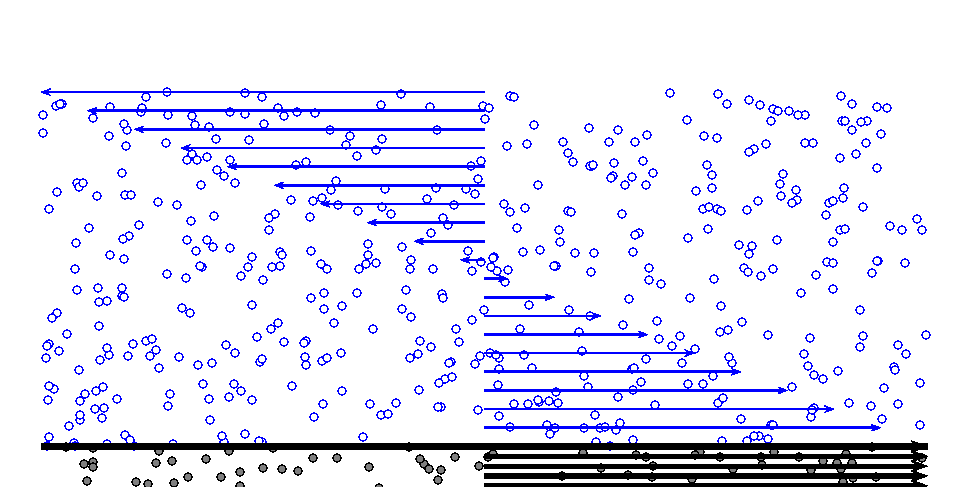
\includegraphics[width=0.5\textwidth]{adaptiveShearForce.pdf}
\caption{Velocities of solvent (blue) and wall particles (grey), shown as arrows.\label{fig:adaptShear}}
\end{figure}

In order to correct this, all particles close to the boundary, i.e. $h < r_{ shear}$, experience a tangential force:
\begin{equation}
F_t^k(h) = C_k\left(\Delta v_t \right) w(h)
\label{eq:adaptive_shear_force}
\end{equation}
with $k$ as the iteration number and the weight function
\begin{equation}
w(h) = \left(1 - \frac{r}{r_{shear}} \right)^{power}
\label{eq:adaptive_sf_weight_fct}
\end{equation}
and the iterative \textit{adaptive force strength}
\begin{equation}
C_{k+1} = C_k + \alpha \Delta v_t
\label{eq:adaptive_force_strength}
\end{equation}

where $\alpha$ is the relaxation parameter, which is set in 'plane.dat'. This parameter could be calculated adaptively in future implementations.\\$\Delta v_t = v_t^{ BC} - v_t^{ est}$. The boundary's velocity is set in plane.dat, and the estimated velocity is extrapolated from the near-boundary velocity profile, which is obtained through local cell averaging.\\After a number of iterations, the particles' velocities approach the boundary's velocity ($\longrightarrow \Delta v_t \approx 0$) so that $F_t^k(h)$ and $C_k$ converge to constant values.\\
\\
\textit{Pressure force; forces read from external file} minimise disturbances in density profile. Particles close to a boundary experience an imbalance of forces, as each of them interacts with a not-fully spherical region of fluid particles, see graphics \ref{fig:wallNeighbours}.

\begin{figure}
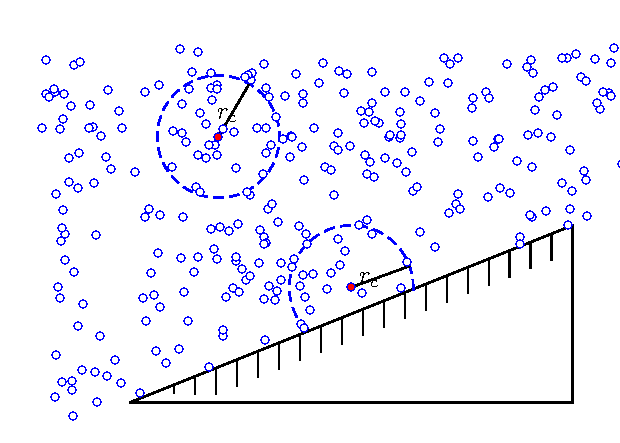
\includegraphics[width=0.5\textwidth]{wallNeighbours.pdf}
\caption{Interactions of solvent particle in bulk and of solvent particle close to wall.\label{fig:wallNeighbours}}
\end{figure}

This option does not consider wall particles and their interactions with the solvent/solute. It replaces the effect of wall particles with imposed conservative and dissipative forces calculated in advance and stored in an external file.\\The conservative force is calculated as:
\begin{equation}
\label{eq:wall_cons_force}
F_p(h) = -n \int_{V_s\backslash V_{ex}(h)} \frac{\partial U}{\partial r} g(r) dV
\end{equation}
with $V_s$ being the interaction sphere's volume, $V_{ex}(h)$ the volume excluded from the sphere by the boundary, and $g(r)$ is the radial distribution function of the specific fluid used in the simulation.

\section{MersenneTwister}

\section{pair styles}

\subsection{pair\_dpd\_thermal}


\subsection{pair\_lj\_own}

Calculation of a Lennard-Jones (LJ) interaction similar as the function LJ/cut with the addition to be able to combine different \glqq special\_bonds\grqq\ and to have different interactions for the internal interactions of a molecule and interactions between different molecules of the same particle id.
\\[2ex]
Syntax:
\\[1ex]
pair\_style lj/own cut-global
\\[2ex]
\textbf{pair\_coeff} iatom jatom $\epsilon$ $\sigma$ which-special-bond \{(cut-local) (\textbf{scale} parameter) (\textbf{molecule} epsilon sigma cut-local)\}

\begin{itemize}
\item \textit{cut-global}: cut-off distance ($r_\mathrm{cutoff}$). Just for smaller particle distances the interaction is calculated. 
\item \textit{iatom, jatom}: atom ids, between which this pair interactions should be calculated
\item $\epsilon$: strength of LJ interaction, see \cref{eq:LJ/own}.
\item $\sigma$: LJ radius, see \cref{eq:LJ/own}
\item which-special-bond: defines special bond for given atom types: value can be 0 or 1 or 2
\item cut-local (optional): changes the cutoff for this pair interaction to cut-local, otherwise it is cut-global.
\item scale: Scale parameter for cutoff
\item molecule: If atoms belong to different molecules, other parameters can be specified.
\end{itemize}

Explanation:
\\[2ex]
The calculated energy between two atoms is:
\begin{equation}\label{eq:LJ/own}
E = 4\epsilon \left[ \left( \frac{\sigma}{r} \right)^{12} -  \left(  \frac{\sigma}{r} \right)^6 \right]
\end{equation}
if $r<r_\mathrm{cutoff}$.
\\[2ex]
For simulations where the special-bonds should be different for different pair interaction, e.g., for a polymer with internal attraction (special\_bonds 1 1 1) and RBCs (special\_bonds 0 0 0), the values can be specified by \textit{which-special-bond}. For \textit{which-special-bond} = 2, the values defined in the input file are taken.
For \textit{which-special-bond} = 1 it is special\_bond 1 1 1 and for  \textit{which-special-bond} it is special\_bond 0 0 0.
\underline{Note}: In the last two cases, the global values in the input file have to be set to a value $\in$ (0.0, 1.0) .
If special\_bonds are set to 0.0 the pair interaction calculation is skipped and for special\_bonds set to 1.0, there is no possibility to distinguish between the three nearest neighbours and all other atoms, because in both cases it would be factor\_lj = 1.
\\[2ex]
Is \textbf{scale} specified, the cutoff the particle distance $r$ is compared to is $r_\mathrm{cutoff} = r_\mathrm{cutoff - specified}*{parameter}$.
The \textit{parameter} has to be smaller than 1.
To set the scale parameter is e.g., usefull if bond creation and/or breakage is wanted.
The distance parameter in these fixes (bond/create, bond/break, bond/create/break) has to be smaller than the defined cutoff, by either cut-global or cut-local, because otherwise the neighbour lists would be wrong, which these fixes use.
By setting a scale parameter, this cutoff for the neighbour list can be chosen larger, than the cut-off for the LJ interaction should be.
\underline{Note}: By increasing the cutoff the computational time increases.
\\[2ex]
For the cases, where the atoms of different molecules should interact differently than the atoms of one molecule, by setting \textbf{molecule} the values for $\epsilon$, $\sigma$ and \textit{cut-local} the interaction between different molecules can be specified separately.
One example are simulations with several polymers with attractive internal interactions between the monomers, where the attraction is not wanted between the monomers of different polymers.
\underline{Note}: Here, cut-local has to be set, it is not optional. Here, the scale parameter does not change the cut-local value set.


\subsection{pair\_sdpd\_full}\label{sec:pair/sdpd/full}

Pair style for interactions by smoothed dissipative particle dynamics (SDPD) with angular momentum conservation.
\\[2ex]
Syntax:
\\[1ex]
pair\_style      sdpd/full $p_0$ $b$ $\alpha$ $T$ group\_sdpd $r_h$ seed group\_fixed $\left< \rho \right>$
\\[1ex]
pair\_coeff      id1 id2 $\rho_0$ $\eta$ $\zeta$

\begin{itemize}
\item $p_0$, $b$, $\alpha$, arguments for pressure equation of state \cref{eq:pressure}.
\item $T$: temperature
\item \textit{group\_sdpd}: group of all particles, which interact by sdpd. Said differently: all particles that should be included for calculation of the particle density $\rho$.
\item $r_h$: cut-off or better said the smoothing length
\item \textit{seed}: seed for random number
\item \textit{group\_fixed}: group of e.g., border particles which do not move
\item $\left< \rho \right>$ is a measured average particle density of the fluid.
\item $\rho_0$: reference particle density
\item $\eta$: dynamic viscosity
\item $\zeta$: bulk viscosity
\end{itemize}

Example:
\\[0.5ex]
pair\_style      sdpd/full 100.0 -80.0 7 0.4 solvent+wall 1.5 8262 wall 3.05018
\\[1ex]
pair\_coeff      1 1 3.0 100.0 ?
\\[2ex]
Explanation:\\
The force $\mathbf{f}_i$ on particle $i$ exerted by all other particles in radius $r_h$ around the particle 
consist of different types of forces
\begin{equation}
\mathbf{f}_i = \sum_{j \neq i} \mathbf{F}^C_{ij} +\mathbf{F}^{D_T} + \mathbf{F}^{D_R} + \mathbf{ \tilde F}_{ij},
\end{equation}
with  $\mathbf{F}^C_{ij}$ the conservative force, $\mathbf{F}^{D_T}$ the translational and $\mathbf{F}^{D_R}$ the rotational dissipative forces, and $\mathbf{ \tilde F}_{ij}$ the random force , given by
%
\begin{align}\label{eq:sdpd_forces}
\mathbf{F}^C_{ij} &= \left( \frac{p_i}{\rho_i^2} + \frac{p_j}{\rho_j^2} \right) F_{ij} \mathbf{r}_{ij}, \nonumber \\
\mathbf{F}^{D_T}_{ij} &= -  \gamma_{ij}^a \left(  \mathbf{v}_{ij} + \frac{ \hat{\mathbf{e}}_{ij}  \left( \hat{\mathbf{e}}_{ij} \cdot \mathbf{v}_{ij} \right) }{3} \right)   - \frac{ 2 \gamma_{ij}^b }{3} \hat{\mathbf{e}}_{ij} \left( \hat{\mathbf{e}}_{ij} 
 \cdot \mathbf{v}_{ij} \right),  \\ 
\mathbf{F}^{D_R}_{ij} & = - \gamma_{ij}^a\frac{\mathbf{ r}_{ij}}{2}\times \left( {\boldsymbol {\omega}}_i+{\boldsymbol{\omega}}_j \right), \nonumber \\ 
\mathbf{ \tilde F}_{ij} &=  \left(  \sigma_{ij}^{a} d\overline{\boldsymbol{\mathcal{W}}}_{ij}^S + \sigma_{ij}^{b} 
\frac{1}{3}tr[d\boldsymbol{\mathcal{W}}_{ij}] \mathds{1} \right) \cdot \frac{\mathbf{\hat e}_{ij}}{dt}, \nonumber
\end{align}
where $p$ is the pressure, $\rho$ is the particle density, $F_{ij}$ calculated from the kernel function $W_{ij}$ (here the Lucy function) as $\nabla_i W_{ij} = -{\mathbf r}_{ij}F_{ij}$  ,$\text{tr}[d\boldsymbol{\mathcal{ W}}_{ij}]$ is the trace of a matrix of independent Wiener increments, 
$d \overline{\boldsymbol{\mathcal{W}}}^{S}_{ij} = d \boldsymbol{\mathcal{W}}^S_{ij} - \text{tr}[d\boldsymbol{\mathcal{W}}_{ij}]\mathds{1}/3$ is the traceless symmetric part.\\
The particle density is given by
%
\begin{equation}\label{eq:rho}
	\rho_i = \sum_j m_j W_{ij}. 
\end{equation}
The friction coefficients are given by
%
\begin{equation} 
	\gamma_{ij}^a = \left( \frac{20\eta}{3}-4\zeta \right)\frac{F_{ij}}{\rho_i\rho_j}, \quad \gamma_{ij}^b = \left( 17\zeta - \frac{40\eta}{3} \right)\frac{F_{ij}}{\rho_i\rho_j},
\end{equation}
% 
and with the random-force coefficient $\sigma_{ij}^{a,b} = 2\sqrt{k_BT\gamma_{ij}^{a,b}}$.
It is important to note that these equations are only valid for $2\eta/3 \le \zeta \le 5\eta /3$, such that the friction coefficients $(\gamma_{ij}^a + 2\gamma_{ij}^b)/3$ and  $\gamma_{ij}^a$ are positive.\\
%
The pressure equation of state used here is
\begin{equation}\label{eq:pressure}
p = p_0 \left( \frac{\rho}{\rho_0} \right)^{\alpha} + b.
\end{equation}
For details see also Ref.~\cite{Mueller_SDPD_2015}.\\[2ex]
Note:\\
In order to use this pair-style the atom style has to be \textit{sdpd} and the integrator has to be \textit{nve/sdpd}.\\
Furthermore, a \textbf{moment of inertia} has to be set in the input-file or the data-file for every particle type similar to the mass.


\subsection{pair\_sdpd}\label{sec:pair/sdpd}

Pair style for interactions by smoothed particle dynamics (SDPD) pair interaction with momentum conservation without taking the bulk viscosity into account as in Subsection \nameref{sec:pair/sdpd/full}.
\\[2ex]
Syntax:
\\[1ex]
pair\_style      sdpd $p_0$ $b$ $\alpha$ $T$ group\_sdpd $r_h$ seed group\_fixed $\left< \rho \right>$
\\[1ex]
pair\_coeff      id1 id2 $\rho_0$ $\eta$\\[2ex]
For details of the parameters see the explanation of Subsection \nameref{sec:pair/sdpd/full}.\\[2ex]
Example:
\\[0.5ex]
pair\_style      sdpd 100.0 -80.0 7 0.4 solvent+wall 1.5 8262 wall 3.05018
\\[1ex]
pair\_coeff      1 1 3.0 100.0
\\[2ex]
Explanation:\\
The forces are the same as above but simplified such that we have one dissipative (random) parameter instead of two. 
It is  
\begin{align}\label{eq:singlep}
	\gamma_{ij} = \gamma^a_{ij} &= \gamma^b_{ij} = \frac{20\eta}{7}\frac{F_{ij}}{\rho_i\rho_j}  \\
  \sigma_{ij} = \sigma^a_{ij} &=\sigma^b_{ij} = 2\sqrt{k_BT\gamma_{ij}}. \nonumber
\end{align}
For details see also Ref.~\cite{Mueller_SDPD_2015}.\\[2ex]
Note:\\
In order to use this pair-style the atom style has to be \textit{sdpd} and the integrator has to be \textit{nve/sdpd}.\\ 
Furthermore, a \textbf{moment of inertia} has to be set in the input-file or the data-file for every particle type similar to the mass.


\subsection{pair\_sdpd\_no\_moment}\label{sec:pair/sdpd/nomoment}

Pair style for smoothed dissipative particle dynamics (SDPD) without angular momentum conservation.
Syntax:
\\[1ex]
pair\_style      sdpd/no/moment $p_0$ $b$ $\alpha$ $T$ group\_sdpd $r_h$ seed group\_fixed $\left< \rho \right>$
\\[1ex]
pair\_coeff      id1 id2 $\rho_0$ $\eta$\\[2ex]
For details of the parameters see the explanation of pair/sdpd/full.\\[2ex]
Example:
\\[0.5ex]
pair\_style      sdpd/no/moment 100.0 -80.0 7 0.4 solvent+wall 1.5 8262 wall 3.05018
\\[1ex]
pair\_coeff      1 1 3.0 100.0
\\[2ex]
Explanation:\\
The forces are very similar to those in \cref{eq:sdpd_forces}; however, the rotational force contribution is excluded.
The conservative force is kept the same, while the dissipative force assumes a coefficient
\begin{equation}
 \gamma_{ij} = 5\eta F_{ij}/(3\rho_i\rho_j)
\end{equation}
using the formulation with a single dissipative parameter as in \cref{eq:singlep}. See also Ref.~\cite{Espanol_SDPD_2003} for further information.\\[2ex]
Note:\\
This pair-style does \textbf{not} require as special atom-style or integrator.

\section{set\_individ}


\section{statistic}

Calculation and output of statistics.
\\[2ex]
\underline{Syntax:}
\\[1ex]
statistic stat-name group-id cyl\_ind n1 n2 n3 stat\_start calc\_each dump\_each (c1 c2 c3 c4 c5 c6) fname

\begin{itemize}
\item \textit{stat-name}: name of the statistic which should be calculated, e.g., center-of-mass (com), velocity (vel). See a full list below.
\item \textit{group-id}: id of group for which statistic should be calculated
\item \textit{cyl\_ind}: $\textbf{0}$ for Cartesian coordinates, {\bfseries 1} for cylindrical coordinates.
\item \textit{n1, n2, n3}: are the number of bins in the three directions: ($x$ $y$ $z$) or ($x$ $r$ $\theta$)
\item \textit{stat\_start}: timepoint for which statistic calculation starts
\item \textit{calc\_each}: calculation of statistic every this many timesteps
\item \textit{dump\_each}: dump a file this many timesteps (first output will be after stat\_start+dump\_each)
\item \textit{c1, c2, c3, c4, c5, c6}: coordinates for the region the statistic is calculated in. To set them is optional. If they are not set, global border domains are used. For details see below.
\item \textit{fname}: output file name. The output looks mostly as: fname.timestep.plt
\end{itemize}

In \textbf{Cartesian coordinates}: c1 = $x_\mathrm{min}$, c2 = $x_\mathrm{max}$, c3 = $y_\mathrm{min}$, c4 = $y_\mathrm{max}$, c5 = $z_\mathrm{min} $ and c6 = $z_\mathrm{max}$.\\
Only particles, which are located in the region from $x_\mathrm{min}$ to $x_\mathrm{max}$ etc. the statistic will be calculated, besides some exceptions.
If they are not set the global border domains are used.
\\[2ex]
In \textbf{cylinder coordinates}: c1 = $x_{min}$, c2 = $x_{max}$, c3 = $y_0$, c4 = $r$, c5 = $z_0$ , c6.\\
$(y_O, z_0)$ is the center of the cylinder and $r$ the radius, thus the cylinder has to be in x-direction.
The parameter c6 is additionally used to distinguish different ways of handling the cylindrical coordinates for some cases.
See, the descriptions of the individual statistics for details and for examples.


\subsection{statistic\_com}

Name: {\bfseries com}\\[2ex]
Example for RBCs in a cylinder:\\[0.5ex]
statistic       com rbc 1 1 250 1 100000 1 100000 0.0 80.2141 0.0 10.0 0.0 0.1 center\_rbc
\\[2ex]
Calculates the center-of-mass (COM) probability distribution for molecules in the specified grid.
Furthermore, the second power of the radius of gyration in all directions and the 3D radius of gyration, the COM velocities in all directions, and the forces in all directions on the COM are calculated (averaged) in the specified grid.
The atoms have to belong to a \textbf{molecule}.
\\[2ex]
Is cyl\_ind = 1 and c6 $\le$ 0.5 the statistic calculation of second power of the radius of gyration, the velocity, and the force is done for Cartesian coordinates (e.g., $f_x$, $f_y$, $f_z$).\\
Is cyl\_end = 1 and c6 $>$ 0.5 the statistic calculation of second power of the radius of gyration, the velocity, and the force is done in cylinder coordinates (e.g., $f_x$, $f_r$, $f_{\theta}$).
\\[2ex]
The output file contains {\bfseries 14} rows.
The first three rows of the output file are the coordinates, either $x$, $y$, $z$ for cyl\_ind = 0 or $x$, $r$, $\theta$ for cyl\_ind = 1 (independent of c6).
The fourth row contains the probability of the com location at the corresponding coordinate (center\_mass), the next 4 rows contain the square of the radius of gyration in all three directions (Rgx2, Rgy2, Rgz2) and the 3D one (Rg2 = Rgx2+Rgy2+Rgz2), the next three rows contain the COM velocity (Vcx, Vcy, Vcz) and the last three rows the force on the COM (Fx, Fy, Fz).


\subsection{statistic\_com\_time}

Name: {\bfseries com/time}\\[2ex]
Example:\\[0.5ex]
statistic       com/time plat 0 1 1 1 100000 1 100 0.0 80.2141 0.0 10.0 0.0 0.1 com\_time
\\[2ex]
Calculation of the average of the center-of-mass (COM) position and the COM velocity for molecules of the specified group.
The specified grid is ignored here.
\\[2ex]
The output are either in Cartesian ($x$, $y$, $z$, $v_x$, $v_y$, $v_z$) or cylinder coordinates ($x$, $r$, $\theta$, $v_x$, $v_r$, $v_{\theta}$) depending on \textit{cyl\_ind}.
\\[2ex]
The number of rows in the output file depends on the number of molecules. 
The first row of the output file is the time of output.
For every molecule, which belongs to the defined group 6 rows follow.
The first 3 rows are the COM position (comx, comy, comz) and the following 3 rows contain the com velocity (com\_velx, com\_vely, com\_velz) in the specified coordinates.
The data is not written to several files, but to the same file.
\\[2ex]
Note: The time between different outputs should not be too large, otherwise this measurement is useless.
Furthermore, depending on the number of particles and the number of outputs the usage of this statistic might be more time consuming than to dump the data more often and to calculate the positions and velocities from the dump file.


\subsection{statistic\_corr}

Name: {\bfseries corr}
\\[2ex]
Calculates the position correlation function.
\\[2ex]
\underline{Syntax:}\\
statistic	corr group cyl\_ind n\_x n\_y calc\_each start\_time dummy dump\_each filename
\begin{itemize}
\item n\_y $\approx$ \#time-lags
\item n\_z exchanged by calc\_each: calculation of statistic every this many timesteps
\end{itemize} 
Here, just Cartesian coordinates are taken into account; cyl\_ind = 0 automatically.
The specified grid is ignored here.
\\[2ex]
The output file contains {\bfseries nx + 1} rows.
The fist row is the time-lag and the next rows the time-dependent position correlation function.


\subsection{statistic\_dens}

Name: {\bfseries dens}
\\[2ex]
Example:\\[0.5ex]
statistic       dens sol 1 1 250 1 100000 1 100000 0.0 80.2141 0.0 10.0 0.0 0.1 dens
\\[2ex]
Calculates the average of the number density and the mass density for the given atom group on the specified grid.
\\[2ex]
The output file contains {\bfseries 5} rows.
The first three rows of the output file are the coordinates, either $x$, $y$, $z$ for \textit{cyl\_ind} = 0 or $x$, $r$, $\theta$ for \textit{cyl\_ind} = 1 (independent of \textit{c6}).
The value of \textit{c6} is ignored.
The fourth row contains the number density and the last row contains the mass density.


\subsection{statistic\_e}

Name: {\bfseries e}
\\[2ex]
Measures the average internal temperature of the particles in the specified atom group on the specified grid.
Note: This statistic can only be used in combination with \textbf{pair\_dpd\_thermal}.
\\[2ex]
The Output consists of {\bfseries 4} rows.
The first three rows of the output file are the coordinates, either $x$, $y$, $z$ for \textit{cyl\_ind} = 0 or $x$, $r$, $\theta$ for \textit{cyl\_ind} = 1 (independent of \textit{c6}).
The value of \textit{c6} is ignored.
The fourth row is the averaged temperature. 


\subsection{statistic\_extension}

Name: {\bfseries extension}
\\[2ex]
Example:
\\[0.5ex]
statistic       extension vwf 0 1 1 1 100000 1 100 0.0 80.2141 -10.0 10.0 -10.0 10.0 ext
\\[2ex]
The (average) extension $R_s = \mathrm{MAX} - \mathrm{MIN}$ of a molecule, the difference between the largest and the smallest position of the particles that belong to one molecule, is measured for all three directions.
Here, just Cartesian coordinates are taken into account, \textit{cyl\_ind = 0} automatically.
The specified grid is ignored here.
\\[2ex]
The number of rows in the output file depends on the number of molecules.
The first row is always the current simulation time.
Then for every molecule 6 rows follow.
The first three of these are the current extensions in all three directions
The following three rows are the averaged extension over the specified time.
Here, the data is constantly written to the same file.
The last three rows are the averaged extension of all molecules.
\\[2ex]
Note: The usage of this statistic might be more time consuming than to dump the data more often and to calculate the extension from the dump-file.


\subsection{statistic\_force}

Name: {\bfseries force}
\\[2ex]
Calculates the average force for all three directions on atoms of the specified group on the specified grid.
\\[2ex]
Here, if cyl\_ind = 1 and c6 $\le$ 0.5 the calculation of the force is done for Cartesian coordinates ($f_x$, $f_y$, $f_z$).
Is cyl\_end = 1 and c6 $>$ 0.5 the calculation of the force is done in cylinder coordinates ($f_x$, $f_r$, $f_{\theta}$).
\\[2ex]
The output file contains {\bfseries 6} rows.
The first three rows of the output file are the coordinates, either $x$, $y$, $z$ for cyl\_ind = 0 or $x$, $r$, $\theta$ for cyl\_ind = 1 (independent of c6).
The last three rows contain the forces for the three directions.


\subsection{statistic\_gyro}

Name: {\bfseries gyro}\\[2ex]
Example\\[0.5ex]
statistic       extension vwf 0 1 1 1 1 1 100 0.0 10.0 0.0 8.0 0.0 8.0 ext
\\[2ex]
Calculates the second power of the radius of gyration $R_g$ of a molecules.
Here, just Cartesian coordinates are taken into account; cyl\_ind = 0 automatically.
The specified grid is ignored here.
\\[2ex]
The radius of gyration is defined as
%
\begin{equation}
 R_g = \sqrt{\frac{1}{2N^2}\sum_{i,j}(\vec{r}_j-\vec{r}_j)^2}
\end{equation}
%
with $N$ the number of monomers and $\vec{r}_i$ the position of monomer $i$.
\\[2ex]
The number of rows in the output file depends on the number of molecules.
The first row is always the current simulation time.
Then for every molecule 4 rows follow.
The first three of these are the second power of the radius of gyration in all three directions (Rgx, Rgy, Rgz).
The next row is the second power of the 3D radius of gyration (Rgx + Rgy + Rgz).
The last 4 rows are always the average over all molecules of the second power of radius of gyration.
Here, the data is constantly written to the same file.


\subsection{statistic\_msd}\label{ssec:stat_msd}

Name: {\bfseries msd}
\\[2ex]

\textbf{Syntax:}\
\\[0.5ex]
statistic	msd group cyl\_ind calc\_each n\_y dummy start\_time dummy dump\_each filename
\begin{itemize}
\item n\_x exchanged by calc\_each: calculation of statistic every this many timesteps
\item n\_y $\approx$ \#time-lags
\end{itemize} 
\textbf{Example:}
\\[0.5ex]
statistic rbc 0 10000 200 66 1000 666 6000000
\\[2ex]
\textbf{Description:}
\\[0.5ex]
Calculates the \textbf{m}ean \textbf{s}quared \textbf{d}isplacement (MSD) of the center of mass (COM).
\\[2ex]
Here, just Cartesian coordinates are taken into account; cyl\_ind = 0 automatically.
The specified grid is ignored here.\\
The MSD is calculated as
%
\begin{equation}
\mathrm{MSD} = \left \langle \left ( \vec{r}_\mathrm{CM}(t_0 + t) - \vec{r}_\mathrm{CM}(t_0) \right ) ^2 \right \rangle _{t_0},
\label{eq:MSD}
\end{equation}
%
with $r_\mathrm{CM}$ the COM position.
\\[2ex]
This module employs
%
\begin{itemize}
\item an average over all $t_0$, meaning all pairs of COM-coordinates that have equal time lags (= delays) $t$ (so short time lags are intrinsically better sampled)
\item on top of that, an exponential mapping of time lags: more values for shorter time lags
\item circular arrays: arrays that, once they have reached their last element, store the next values from the beginning onwards (see the modulo operator \%)
\end{itemize}
%
In the first stage of this function, it 'collects' sufficient data (the center of mass positions at certain time steps) and in the second stage, the correlations are calculated. After enough data has been collected, the function replaces sequentially the values within the circular arrays, so everytime, new correlations can be calculated.
\\[2ex]
Note: \cref{eq:MSD} can be analyzed to obtain the type of motion: for short time lags $t$, numerical motion is ballistic and $\mathrm{MSD} \propto t^2$.
For larger time lags, in case of pure diffusion, \cref{eq:MSD} is linearly dependent on $t$ and the translational diffusion coefficient can be fitted.
For the post-processing: The transition time \textit{ballistic} $\longrightarrow$ \textit{diffusive} can be obtained by using double logarithmic scale and one linear and one quadratic fit function.:
%
\begin{equation}
\mathrm{MSD} = 6 \cdot D_{\mathrm{trans}} \cdot t
\label{MSD_diffusion}
\end{equation}
%
The factor of 6 for the case of 3 dimensions.
\\[2ex]
The output file contains {\bfseries 2} rows.
The fist row is the time-lag and the second the time-dependent MSD.

\subsection{statistic\_rho}

Name: {\bfseries rho}
\\[2ex]
Example\\[0.5ex]
statistic       rho nocell 1 1 250 1 100000 1 100000 0.0 80.2141 0.0 10.0 0.0 0.1 rho
\\[2ex]
Calculates the average of the particle density $\rho$ on the specified grid.
See \cref{eq:rho} for the definition of $\rho$.
\\[2ex]
The output file contains {\bfseries 4} rows.
The first three rows of the output file are the coordinates, either $x$, $y$, $z$ for cyl\_ind = 0 or $x$, $r$, $\theta$ for cyl\_ind = 1 (independent of c6).
The fourth row contains $\rho$.
\\[2ex]
Note:\\
This function can only be used for simulations with the pair interaction sdpd/full, sdpd, or sdpd/no/moment.


\subsection{statistic\_stress}

Name: {\bfseries stress}

Calculates the average stress tensor for the specified grid.
Here, just Cartesian coordinates are taken into account; cyl\_ind = 0 automatically.
\\[2ex]
The statistic outputs either 2 or 4 files.
The latter is the case, if the given group is connected by bonds, angles, or dihedrals.\\
The output files contain {\bfseries 15} rows.
The first output file is \glqq atom1\_fname.timestep.plt\grqq.
The second output file is \glqq atom2\_fname.timestep.plt\grqq.
The third output file is \glqq poly1\_fname.timestep.plt\grqq.
The fourth output file is \glqq poly2\_fname.timestep.plt\grqq.
The first three rows of the output file are the coordinates $x$, $y$, $z$.
The next 6 rows are the entries of the first tensor.
The next 6 rows are the entries of the second tensor.


\subsection{statistic\_vcorr}

Name: {\bfseries vcorr}
\\[2ex]
Calculates the velocity correlation function of the center-of-mass velocity of the given group.
\\[2ex]
\underline{Syntax:}\\
statistic	corr group cyl\_ind calc\_each n\_y dummy start\_time dummy dump\_each filename
\begin{itemize}
\item n\_x exchanged by calc\_each: calculation of statistic every this many timesteps
\item n\_y $\approx$ \#time-lags
\end{itemize} 
Here, just Cartesian coordinates are taken into account; cyl\_ind = 0 automatically.
The specified grid is ignored.\\
The correlation is calculated as
\begin{equation}
\mathrm{vcorr} = \left \langle \vec{v}(t_0 + t) \vec{v}(t_0)  \right \rangle _{t_0},
\label{eq:vcorr}
\end{equation}
\\[2ex]
The output file contains {\bfseries 2} rows.
The fist row is the time-lag and the second row the time-dependent velocity correlation function.
\\[2ex]
See also: Subsection \nameref{ssec:stat_msd}


\subsection{statistic\_vel}

Name: {\bfseries vel}
\\[2ex]
Example:
\\[0.5ex]
statistic       vel sol 0 1 600 1 10 1 100000 0.0 10.0 0.0 8.0 0.0 8.0 vel
\\[2ex]
Calculates the average of the velocity in all directions on the specified grid for the given atom group.
\\[2ex]
Is cyl\_ind = 1 and c6 $\le$ 0.5 the statistic calculation is done for Cartesian coordinates ($v_x$, $v_y$, $v_z$).
Is cyl\_end = 1 and c6 $>$ 0.5 the statistic calculation is done in cylinder coordinates ($v_x$, $v_r$, $v_{\theta}$).
\\[2ex]
The output file contains {\bfseries 6} rows.
The first three rows of the output file are the coordinates, either $x$, $y$, $z$ for cyl\_ind = 0 or $x$, $r$, $\theta$ for cyl\_ind = 1 (independent of c6).
The next three rows contain the averaged velocities (v\_x, v\_y, v\_z).


\section{COPY}

Here we have some files that are not needed ad the moments but are there

\subsection{single\_triangle}

\subsection{statistic\_DLS}

Calculates the \textbf{d}ynamic \textbf{l}ight \textbf{s}cattering.

Based on statistic\_SLS, this module calculates the correlation function of the scattering amplitudes in a similar fashion like statistic\_msd:
%
\begin{equation}
S(\vec{q}, t) = < A(\vec{q},t_0)A^*(\vec{q},t_0+t) >_{t_0}
\label{eq:DLS}
\end{equation}
%
This module employs
%
\begin{itemize}
\item an average over all $t_0$, meaning all pairs of scattering amplitudes that have equal time lags (= delays) $t$ (so short time lags are intrinsically better sampled)
\item an average over orientations of $\vec{q} = \vec{k}_{in} - \vec{k}_{s}$, which have to be supplied in an external file. This file shall be named \textit{q\_orientations.dat} and contain the number of vectors (first line) and sequentially, the three coordinates of each vector in each line.
\item linear mapping of time lags (in contrast to statistic\_msd)
\end{itemize}
%
It is possible to continue another \textit{LAMMPS} run with the data already calculated by choosing the input parameter output\_ind $\neq 0$. In the case output\_ind$=1$, output files are generated; in the case output\_ind$>1$, output files are both read in and generated. If neither shall be used, set output\_ind$=0$.

The output is structured as follows: time lag t \quad q-magnitude \quad $\mathfrak{R} (S)$ \quad $\mathfrak{I} (S)$.

\underline{Syntax:} statistic	DLS group cyl\_ind calc\_each \#time-lags n\_q\_mag start\_time output\_ind dump\_each filename


\subsection{statistic\_SLS}

Calculates the \textbf{s}tatic \textbf{l}ight \textbf{s}cattering on triangulated objects. The theoretical basis is the Rayleigh Gans Debye - approximation. Multiple scattering is neglected as well as special considerations of dielectric constants. The quantity output is the complex bulk scattering amplitude:
%
\begin{equation}
\label{eq:SLS}
A_b(\vec{q})=\int_V e^{i\vec{q} \cdot \vec{r}} dV
\end{equation}
%
alongside the magnitude of the momentum transfer vector $\vec{q} = \vec{k}_{in} - \vec{k}_{s}$. In case of non-spherical particles, changing the orientation of $\vec{q}$ leads to a different course of $A_b(q)$.

This module employs
%
\begin{itemize}
\item the module \textit{single\_triangle.cpp} which calculates the scattering amplitude of one triangle and according to $\vec{q}$
\item circular arrays: arrays that, once they have reached their last element, store the next values from the beginning onwards (see the modulo operator \%)
\item MPI-parallelisation for the contributions of the different triangles
\end{itemize}
%
The maximum value for the magnitude of the momentum transfer vector $\vec{q}$, $q_{max}$, is calculated such that $q_{max} \cdot l_0 = 2 \pi$, with $l_0$ being the smallest length scale of the object\footnote{As exclusively triangulated objects are permitted, $l_0$ is the average triangle length.}. The number of different magnitudes for $\vec{q}$, $n_{q-mag}$, is input (see below). With these values, the difference of adjacent $|\vec{q}|$s is calculated.

\underline{Syntax:} statistic	SLS group cyl\_ind calc\_each \#time-lags n\_q\_mag start\_time dummy dump\_each filename

\section{vector}


\section{MAKE/MINE}


\section{USER-SDPD}

% ? Dmitry?\\
% ?What is importan?


% \subsubsection{Other}
% 
% [atom\_vec\_individual.cpp, atom\_vec\_individual.h but not used, stored in OLD\_FILES/]

\chapter{Tools}

\section{Analyser for analysing the statistic}

In the folder \glqq Analyser/ \grqq tools to analyse the statistic data are provided.
The analyser is for statistic data, where something is averaged on the grid, e.g., com, vel, dens etc.
\\[1ex]
Syntax:\\[0.5ex]
./analyser stat.dat fname \#columns-3
\begin{itemize}
\item \textit{analyser}: the executable
\item \textit{stat.dat}: input file which is described below
\item \textit{fname}: file name as given in the LAMMPS input file
\item \textit{\#columns-3} number of columns in the statistic files minus 3, because the $x,y,z$-columns are always there.
\end{itemize}
Example:\\[0.5ex]
./analyser stat.dat center\_rbc 11
\\[2ex]
In 3D there exist different possibilities to average
\begin{itemize}
\item The center-of-mass data, therefore the code in the folder \glqq3D/Center\_mass/\grqq\ has to be used.
\item In order to average data from different partition separately use the code in \glqq3D/Part\_Separate/\grqq. The output is a file fname\#part\_tot.plt for every partition, with \#part the number of partition
\item In order to average data from different partitions use the code in \glqq3D/Part\_Together/\grqq. The output is one file with the name fname\_tot.plt
\end{itemize}
The stat.dat file is similar for all cases and looks e.g., as follows:
\begin{table}[h!]
  \begin{tabular}{ll}
    32 1 1       & - partitions: tot number, start, interval\\
20 100000 100000 & - stat outputs: tot number, start, interval\\
1 40 1           & - domain division: nx, ny, nz\\
1.0 1.0 1.0 1.0  & - scale: x\_scale, y\_scale, z\_scale, dat\_scale\\
1                & - standard deviation: 1 - calculate, 0 -no\\
  \end{tabular}
\end{table}
The meaning of the lines is 
\begin{enumerate}
  \item 
  \begin{itemize}
    \item first number(32): total number of partition
    \item second number (1): the smallest number of a partition, 
    \item third number (1): interval between the numbers of the partitions
  \end{itemize} 
\item
\begin{itemize}
    \item first number(20): number of output files
    \item second number (100000): timestep of the first file (stat\_start+dump\_each from the LAMMPS input file)
    \item third number (100000): timestep-interval of the outputs (dump\_each from LAMMPS input file).
  \end{itemize}
\item domain division. Same numbers as in the LAMMPS input file for \textit{n1 n2 n3}
\item scaling parameter for the x-coordinates, y-coordinates, z-coordinates and the data.
\item Calculation of the standard deviation: yes (1) or no (0)
\end{enumerate}
Note: If in the second row the numbers cover more than you have output files, the averaging is nevertheless done correctly.

\section{compiling \& running LAMMPS personal}
To compile our group version of LAMMPS, you find the source code in the repository folder \textit{/blood/lammps\_personal/src/}.
\newline
Delete old object files:\\
\textbf{make clean-all}
\newline
\textbf{make clean-machine}
\newline
compile LAMMPS and generate executable 'lmp\_iff':\\
\textbf{gmake iff}
\newline
run LAMMPS:\\
\textbf{mpirun -np \textit{Cores} lmp\_iff \textless \quad \textit{input\ file}}

In general, the supercomputers have different architectures.\\For the supercomputer binaries, 'iff' has to be replaced in the above commands.

\section{data\_domain}
\label{sec:data_domain}
Before running a simulation, an initial configuration of particles (called 'atoms' in \textit{LAMMPS}) has to be generated.\\This can be done by writing a parameter file called \textit{domain.dat} and running the program \textit{data\_domain}.
\subsection{data\_domain - code}
Its code is in the repository at \textit{~/blood/Data\_File\_Creator/} and is compiled by\\ \textit{g++ data\_domain.cpp -o data\_domain}\\\textit{data\_domain} always processes the file called \textit{domain.dat} - no matter what you give as command-line parameter.\\It creates a file called \textit{data.out} with all the initial coordinates, momenta, etc. This is read by \textit{LAMMPS}; specified in the input file by\\ \textit{read\_data data.out}

\subsection{domain.dat - parameter file}
\textbf{Syntax of \textit{domain.dat}:}
\begin{itemize}

\item $  atom\_types \quad   individ\_ind $
	\begin{itemize}
	\item number of atom types in total (from single atoms, polymers, objects, borders)
	\item 0 = no; 1 = yes: index for the use of individual bonds/angles/dihedrals
	\end{itemize}

\item $  mass\_ind \quad   mass_1 \quad   mass_2 ... $
	\begin{itemize}
	\item $ mass\_ind$ = 1: read individual masses
	\item $ mass_i$: mass for atom type $i$; the number of masses should match the number of atom types
	\end{itemize}

\item $  moment\_ind \quad   moment_1 \quad   moment_2 ... $
	\begin{itemize}
	\item $ moment\_ind$ = 1: read individual moments
	\item $ moment_i$: moment for atom type $i$; the number of moments should match the number of atom types
	\end{itemize}

\item $ x_{lo} \quad x_{hi} \quad y_{lo} \quad y_{hi} \quad z_{lo} \quad z_{hi} $ \\
	{ global box size; cuboid shape}

\item $num\_atom\_domains$ \\
	{Number of atom domains. The next $num\_atom\_domains$ lines describe the different domains of single particles. Each of them has the following syntax:}

\item $ atom\_type \quad cyl\_ind \quad random\_ind \quad x_{lo} \quad x_{hi} \quad y_{lo}(y_c) \quad y_{hi}(r\_min) \quad z_{lo}(z_c) \quad z_{hi}(r\_max) \quad n_x(n\_rand) \quad n_y \quad n_z $
	\begin{itemize}
	\item $atom\_type$: in the present domain, all particles are of this type
	\item $cyl\_ind$ = 0 or 1: cylindrical domain = cylindrical arrangement of particles
	\item $random\_ind$ = 0 or 1: random arrangement of particles
	\item the next parameters describe the domain size. $c$ and $r$ for the cylindrical option (centre and radius; minimum and maximum: for a hollow cylinder)
	\item $n_i$: number of atoms in each direction; $n_x \cdot n_y \cdot n_z = n\_total$. If random, only the first parameter is used $n\_rand = n\_total$.
	\end{itemize}

\item $num\_polymer\_domains$ \\
	{Number of polymer domains. The next $num\_polymer\_domains$ lines describe the different domains of polymers. Each of them has the following syntax:}

\item $ atom\_type \quad bond\_type \quad cyl\_ind \quad random\_ind \quad x_{lo} \quad x_{hi} \quad y_{lo}(y_c) \quad y_{hi}(r\_min) \quad z_{lo}(z_c) \quad z_{hi}(r\_max)$\\$ n_x(n\_rand) \quad n_y \quad n_z \quad bead\_num \quad r_{eq} \quad r\_sph \quad linear$
	\begin{itemize}
	\item Designed analogously to the atom domains.
	\item The first polymer point will be always at the center points.
	\item $linear = 0$: random walk, if $r\_sph>0.0$ will try to generate it within the sphere, so do not set it too small
	\item $linear = 1,2,3$: aligned with x,y,z respectively.
	\item $cyl\_ind = 2$: on a cylinder plus a polymer is rotated to get aligned with the cylinder radius
	\end{itemize}

\item $num\_object\_domains$ \\
	{Number of object domains. The next $num\_object\_domains$ lines describe the different domains of objects. Each of them has the following syntax:}

\item $atom\_type \quad bond\_type \quad angle\_type \quad dihedral\_type \quad cyl\_ind \quad random\_ind \quad x_{lo} \quad x_{hi} \quad y_{lo}(y_c)$\\$\quad y_{hi}(r\_min) \quad z_{lo}(z_c) \quad z_{hi}(r\_max) \quad n_x(n\_rand) \quad n_y \quad n_z \quad r\_scale \quad file\_name$
	\begin{itemize}
	\item Designed analogously to the atom domains.
	\item $cyl\_ind = 2$: on a cylinder plus an object is rotated to get aligned with the cylinder radius
	\item $r\_scale$: start with the object being scaled by this factor; in the following time steps, the object rescales to its original shape. Useful for dense packing; starting with small objects.
	\item $file\_name$: name of the input file containing the object information (coordinates, bonds, (tri)angles, dihedrals etc.); see below \ref{syn:object_file}
	\end{itemize}

\item $num\_border\_domains$ \\
	{Number of border domains. The next $num\_border\_domains$ lines describe the different domains of borders. Each of them has the following syntax:}

\item $atom\_type \quad cyl\_ind \quad x_{lo} \quad x_{hi} \quad y_{lo}(y_c) \quad y_{hi}(r\_min) \quad z_{lo}(z_c) \quad z_{hi}(r\_max)$\\$shift_x \quad shift_y \quad shift_z \quad linear \quad file\_name$
	\begin{itemize}
	\item Designed analogously to the atom domains.
	\item $shift$: The border file has limited size. Maybe it starts at position 0.0 and ends at 5.0, but you want to put it into your box starting at 16.0. This parameter makes a global translation of the border.
	\item $linear = 1$: no coordinate exchange
	\item $linear = 2$: exchange x and y
	\item $linear = 3$: exchange x and z
	\item $file\_name$: name of the input file containing the border information
	\end{itemize}

\end{itemize}

\textbf{Example:}\\ \\
For a RBC (enclosing an inner fluid differing from the outer fluid) in a cylindrical, solid tube:\\
4 1\\
1 1.0 3.0 2.0 1.0\\
1 1.0 1.0 1.0 1.0\\
0.0 50.0 -13.53 13.53 -13.53 13.53\\
2\\
1 1 1 3.0 49.9 0.0 1.0 0.0 12.42 294412 0 0\\
3 1 1 1.2 1.8 0.0 1.3033 0.0 3.5 1112 0 0\\
0\\
1\\
2 1 1 1 0 0 1.5 1.5 0.0 0.0 0.0 0.0 1 1 1 1.0 \~{}/blood/Templates/3D/rbc\_3000\_def0.96\_x\_D8.dat\\
1\\
4 1 0.0 50.0 0.0 12.5212 0.0 13.5212 0.0 0.0 0.0 1 \~{}/blood/Border\_files/SDPD/box\_100x50x50\_n12\_p100\_b-80\_g7\_et100\_T0.2\_rc1.0\\

There are in total four different atom types: the outer fluid (type 1), the inner fluid (3), the membrane vertices (2) and the border particles (4) (the atoms that make up the tube).\\

\textbf{Description:}\\ \\
This is the parameter file for the initial set-up/configuration. You specify the size of the whole simulation box, the number of atoms, objects (like RBCs), polymers and borders (like solid walls).\\Objects and borders are more complicated so they have to be provided by an external file. For the object-file syntax, see below \ref{syn:object_file}. The border-files are the dump-files of a preceeding \textit{LAMMPS}-simulation run, which generated this border. Preceeding and present simulation have to match in parameters as density, conservative interaction, temperature and cutoff radius.\\The atom type, which has to be specified for each domain, [no matter if single atoms, polymers, objects or borders, ] corresponds to the types used in \textit{LAMMPS}' group command.\\The purpose of multiple (atom, polymer etc.) domains is that you can have different types or arrangements within one simulation box. 
\\ \\
\textbf{Syntax of object file:}
\label{syn:object_file}
\begin{itemize}
\item $num\_atoms \quad num\_bonds \quad num\_angles \quad num\_dihedrals$
\item $ind\_atom\_type \quad ind\_bond\_type \quad ind\_angle\_type \quad ind\_dihedral\_type$\\
	{0 - no individual types, 1 - must define individual types}
\item $ind\_bond\_length \quad ind\_angle\_area \quad ind\_dihedral\_angle$\\
	{0 - no individual values, 1 - must add individual values as last column (after the bond-/angle-/dihedral-partners)}
\item $num\_atoms$ lines for the atoms' coordinates
	\begin{itemize}
	\item syntax: if $ind\_atom\_type=0$: ($x \quad y \quad z$)
	\item syntax: if $ind\_atom\_type=1$: ($atom\_type \quad x \quad y \quad z$)
	\end{itemize}
\item $num\_bonds$ lines for the bonds-partners' indices:
	\begin{itemize}
	\item syntax: if $ind\_bond\_type=0$: ($p_1 \quad p_2$)
	\item syntax: if $ind\_bond\_type=1$: ($bond\_type \quad p_1 \quad p_2$)
	\item syntax: if $ind\_bond\_length=1$: ($p_1 \quad p_2 \quad l_0$)
	\end{itemize}
\item $num\_angles$ lines for the angles-partners' indices:
	\begin{itemize}
	\item syntax: if $ind\_angle\_type=0$: ($p_1 \quad p_2 \quad p_3$)
	\item syntax: if $ind\_angle\_type=1$: ($angle\_type \quad p_1 \quad p_2 \quad p_3$)
	\item syntax: if $ind\_angle\_area=1$: ($p_1 \quad p_2 \quad p_3 \quad A_0$)
	\end{itemize}
\item $num\_dihedrals$ lines for the dihedrals-partners' indices:
	\begin{itemize}
	\item syntax: if $ind\_dihedral\_type=0$: ($p_1 \quad p_2 \quad p_3 \quad p_4$)
	\item syntax: if $ind\_dihedral\_type=1$: ($dihedral\_type \quad p_1 \quad p_2 \quad p_3 \quad p_4$)
	\item syntax: if $ind\_dihedral\_angle=1$: ($p_1 \quad p_2 \quad p_3 \quad p_4 \quad \alpha_0$)
	\end{itemize}
\end{itemize}

%%%%%%%%%%%%%%%%%%%%%%%%%%%%%%%%%%%%%%%%%%%%%%%%%%%%%%%%%%%%%%%%%%%%%%%%%%%%%%%%%%%%%%%%%%%%%%%%%%%%%%%%%%%%%%%%%%%%%%%%%%%%%%%%%%%%%%%%%%%%%%%%
\bibliography{paper.bib} 
\bibliographystyle{unsrt}
\end{document}

